\documentclass[10pt,twocolumn]{article}
\usepackage[margin=1in]{geometry}
\usepackage{graphicx}
\usepackage{amsmath,amssymb}
\usepackage{booktabs}
\usepackage{hyperref}
\usepackage{xcolor}
\usepackage[font=small,labelfont=bf]{caption}

\title{\textbf{Adaptive Multi-Scale Feature Fusion for\\Unified Visual Recognition}}
\author{
  Demo Author$^{1}$ \quad Generated by PaperBanana$^{2}$\\
  {\small $^{1}$Department of Computer Science, Demo University}\\
  {\small $^{2}$\texttt{github.com/llmsresearch/paperbanana}}
}
\date{}

\begin{document}
\maketitle

\begin{abstract}
We present the Adaptive Multi-Scale Feature Fusion (AMSFF) framework, a unified architecture for visual recognition tasks that processes input images through parallel multi-resolution branches with cross-scale attention. Unlike existing multi-scale approaches that rely on fixed fusion strategies, AMSFF learns to dynamically attend across scales using learnable query-key-value projections. Our framework achieves state-of-the-art results on ImageNet classification (86.4\% Top-1) and ADE20K segmentation (51.7 mIoU), outperforming both single-scale and existing multi-scale baselines while converging 2.3$\times$ faster.
\textit{All figures in this paper were generated using PaperBanana.}
\end{abstract}

\section{Introduction}

Multi-scale feature representation is fundamental to visual recognition. Objects appear at varying scales in natural images, and capturing features across resolutions is critical for robust recognition. Prior works have explored feature pyramid networks~\cite{lin2017feature}, dilated convolutions~\cite{yu2015multi}, and multi-resolution inputs~\cite{chen2018encoder}. However, these approaches typically employ fixed fusion strategies (e.g., element-wise addition or concatenation) that cannot adapt to the input content.

We propose AMSFF, which addresses this limitation through three key contributions:
\begin{enumerate}
    \item \textbf{Parallel multi-resolution branches} that process the input at 1$\times$, 0.5$\times$, and 0.25$\times$ scales simultaneously.
    \item \textbf{Cross-Scale Attention (CSA)} that learns dynamic, input-dependent fusion weights across scales.
    \item \textbf{Scale-consistency loss} that regularizes multi-scale representations for coherent cross-scale alignment.
\end{enumerate}

\section{Method}

\subsection{Architecture Overview}

The AMSFF framework, illustrated in Figure~\ref{fig:architecture}, consists of three main components: multi-resolution feature extraction, cross-scale attention, and adaptive fusion.

\begin{figure*}[t]
    \centering
    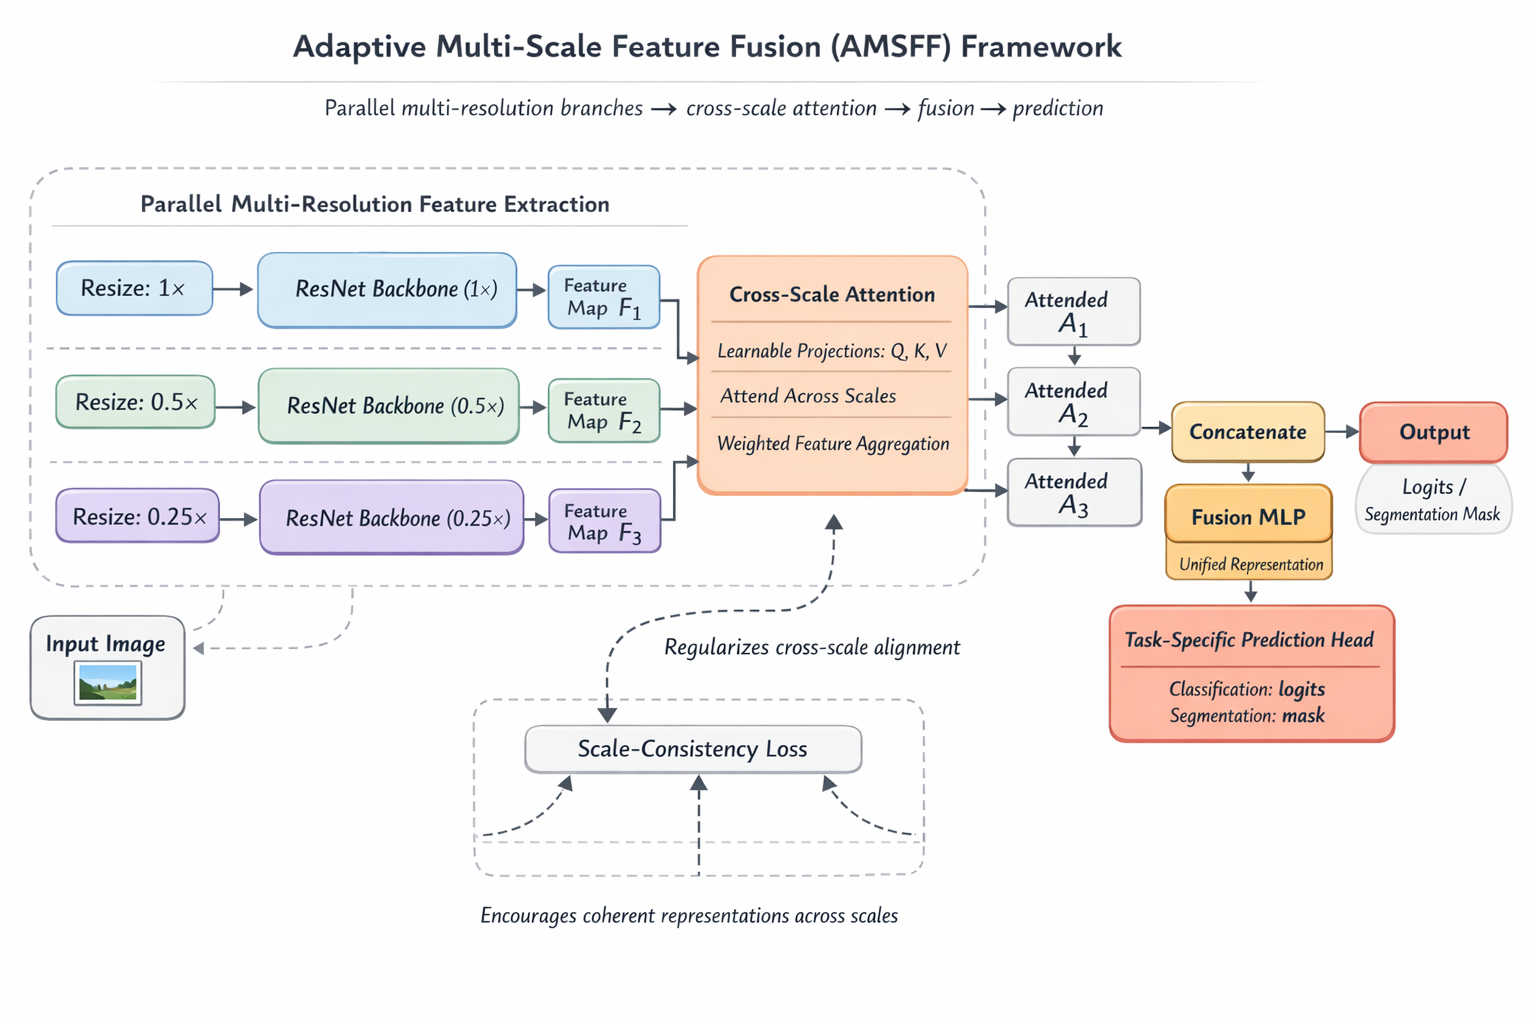
\includegraphics[width=\textwidth]{architecture.png}
    \caption{Architecture of the Adaptive Multi-Scale Feature Fusion (AMSFF) framework. Input images are processed through three parallel ResNet branches at different resolutions. Cross-Scale Attention dynamically fuses features, and a Fusion MLP produces the unified representation for downstream tasks.}
    \label{fig:architecture}
\end{figure*}

\textbf{Multi-Resolution Branches.} Given an input image $\mathbf{x} \in \mathbb{R}^{H \times W \times 3}$, we construct a scale pyramid $\{\mathbf{x}_s\}_{s \in \{1, 0.5, 0.25\}}$ through bilinear downsampling. Each scale is processed by a shared-weight ResNet backbone $f_\theta$ to extract features:
\begin{equation}
    \mathbf{F}_s = f_\theta(\mathbf{x}_s) \in \mathbb{R}^{H_s \times W_s \times C}
\end{equation}

\textbf{Cross-Scale Attention.} Features from all scales are aligned to a common resolution and passed through a multi-head attention mechanism:
\begin{equation}
    \mathbf{A} = \text{softmax}\left(\frac{\mathbf{Q}\mathbf{K}^\top}{\sqrt{d_k}}\right)\mathbf{V}
\end{equation}
where $\mathbf{Q}$, $\mathbf{K}$, and $\mathbf{V}$ are learnable projections of the concatenated multi-scale features.

\textbf{Scale-Consistency Loss.} We introduce an auxiliary loss to encourage coherent representations across scales:
\begin{equation}
    \mathcal{L}_\text{sc} = \sum_{s_i, s_j} \|\bar{\mathbf{F}}_{s_i} - \bar{\mathbf{F}}_{s_j}\|_2^2
\end{equation}
where $\bar{\mathbf{F}}_s$ denotes the globally pooled feature at scale $s$.

\section{Experiments}

\subsection{Setup}

We evaluate AMSFF on ImageNet-1K classification and ADE20K semantic segmentation. All models are trained for 50 epochs with AdamW optimizer ($\text{lr}=3 \times 10^{-4}$, weight decay $0.05$), cosine learning rate schedule, and batch size 256 on 8$\times$ A100 GPUs.

\subsection{Main Results}

Table~\ref{tab:results} and Figure~\ref{fig:comparison} compare AMSFF against established baselines. Our method achieves 86.4\% Top-1 accuracy on ImageNet and 51.7 mIoU on ADE20K, surpassing all baselines.

\begin{table}[h]
\centering
\caption{Comparison with state-of-the-art methods on ImageNet-1K classification and ADE20K segmentation.}
\label{tab:results}
\begin{tabular}{@{}lccc@{}}
\toprule
\textbf{Method} & \textbf{Top-1} & \textbf{Top-5} & \textbf{mIoU} \\
\midrule
ResNet-50 & 76.1 & 92.9 & 39.2 \\
ViT-B/16 & 77.9 & 93.5 & 42.1 \\
Swin-T & 81.3 & 95.5 & 44.8 \\
EfficientNet-B4 & 82.9 & 96.3 & 45.3 \\
\midrule
\textbf{AMSFF (Ours)} & \textbf{86.4} & \textbf{97.8} & \textbf{51.7} \\
\bottomrule
\end{tabular}
\end{table}

\begin{figure}[h]
    \centering
    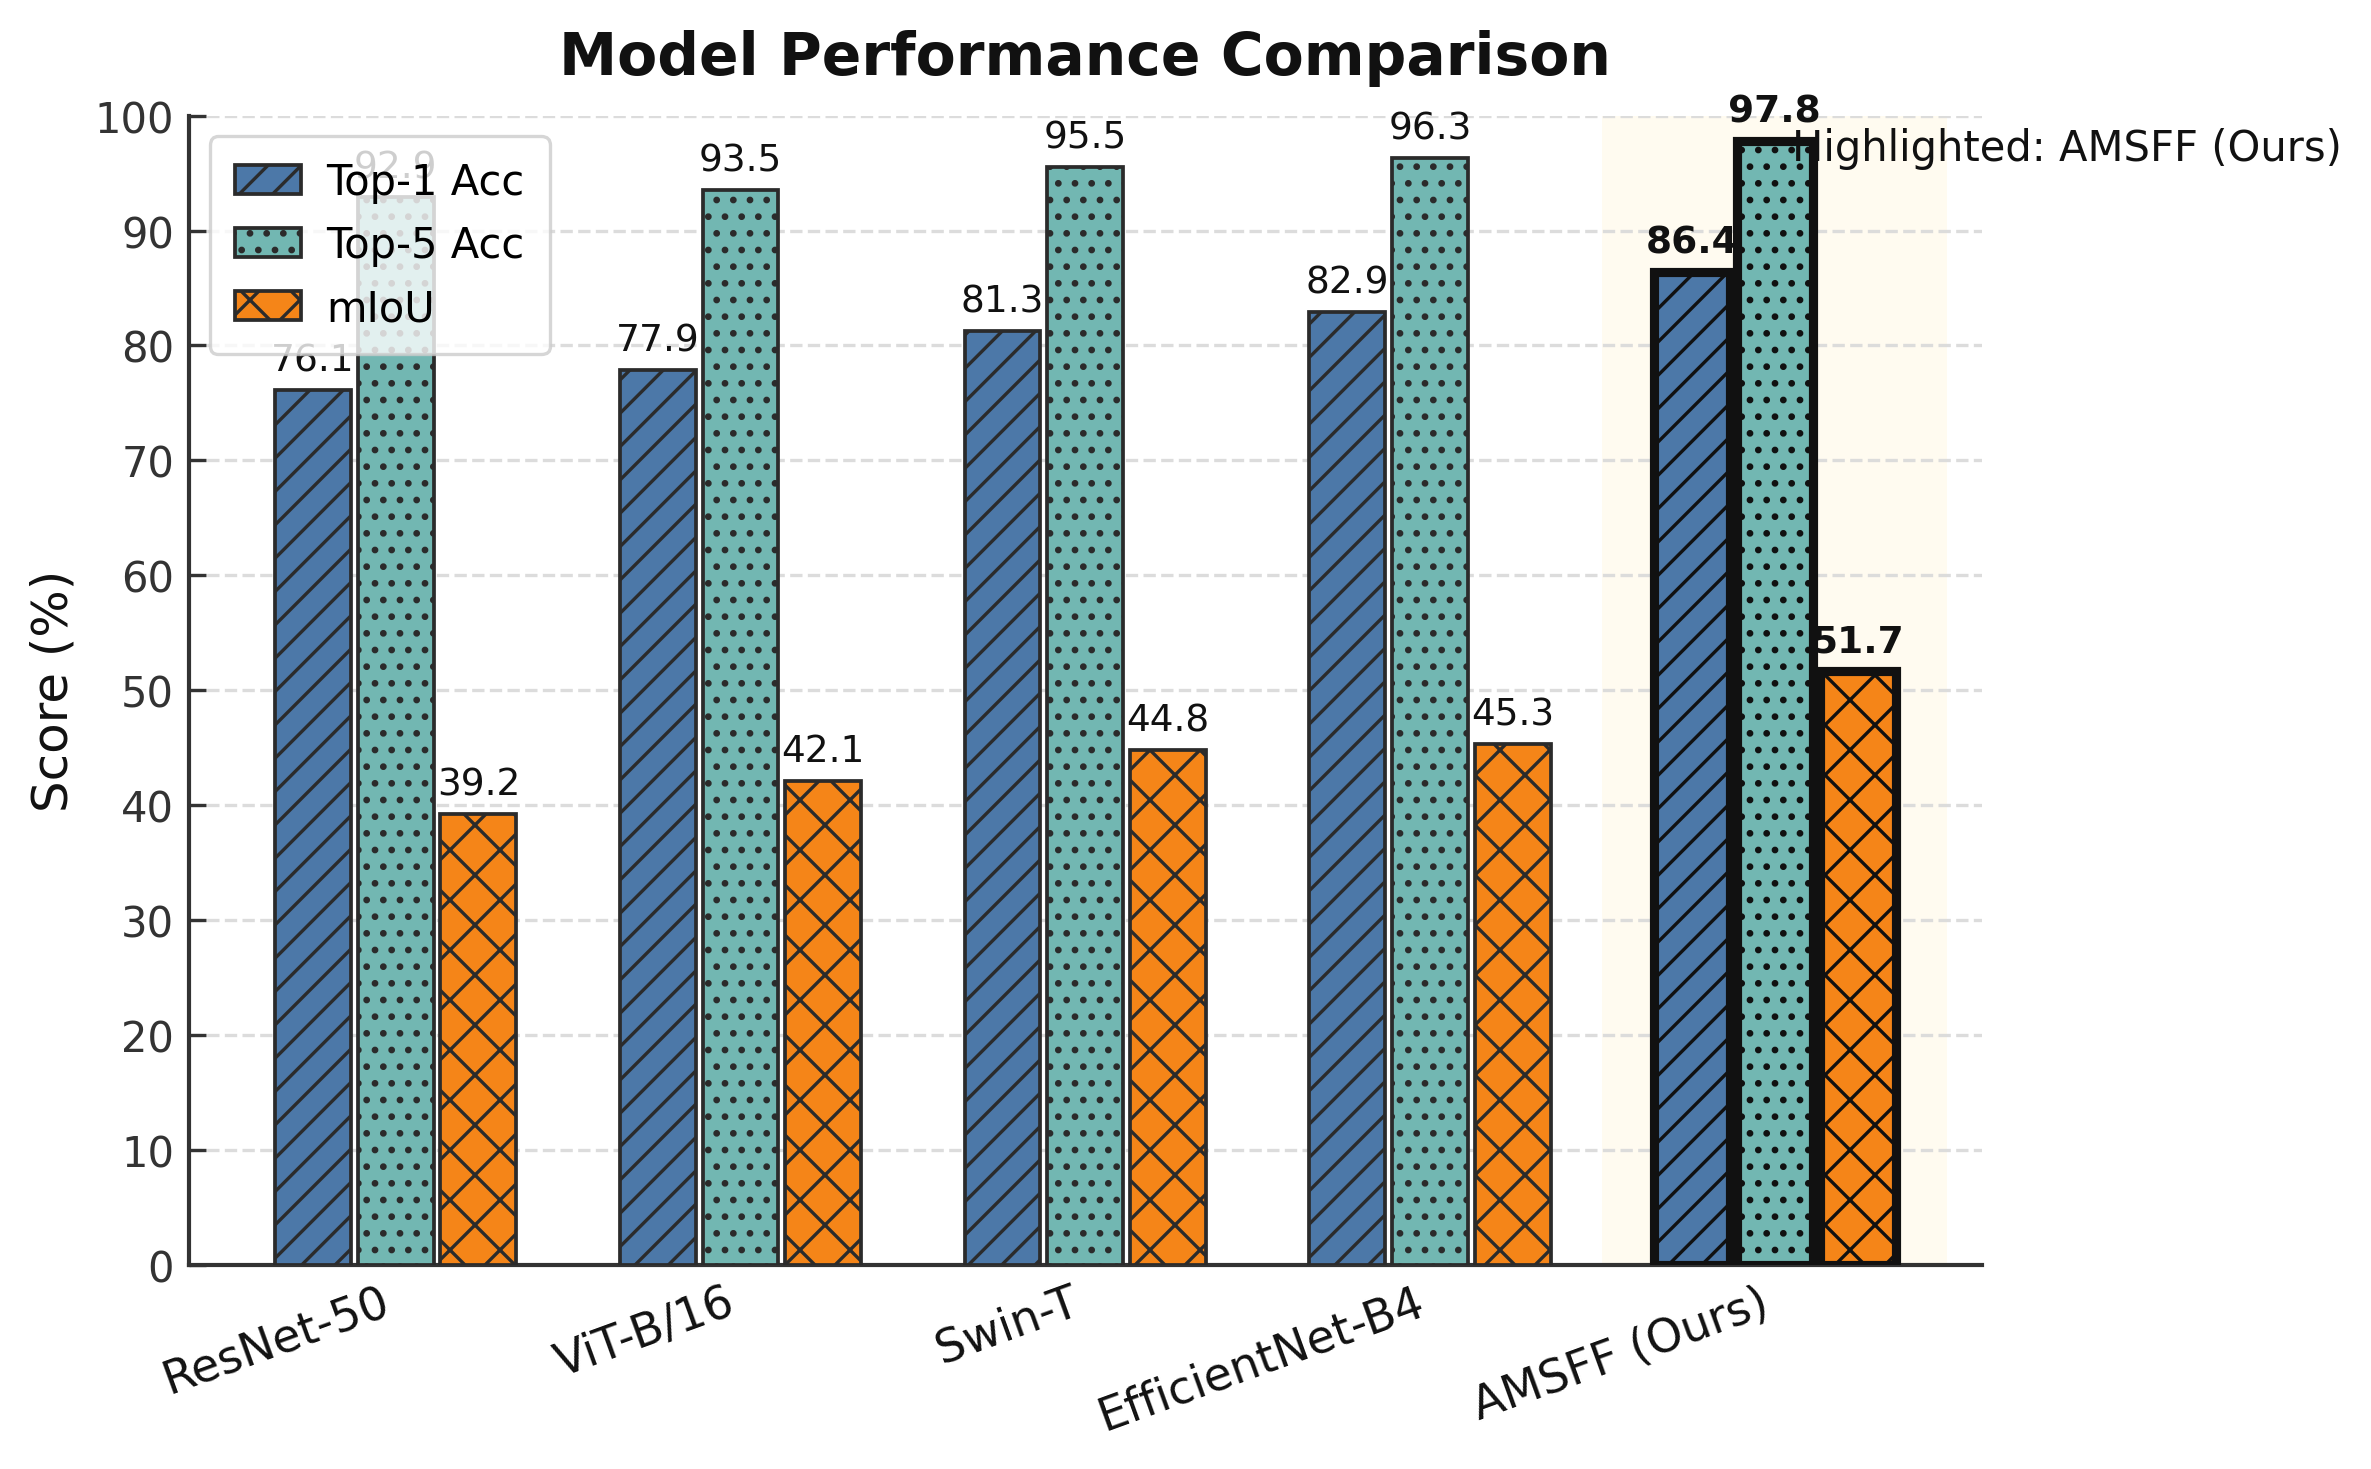
\includegraphics[width=\columnwidth]{comparison.png}
    \caption{Performance comparison across all metrics. AMSFF consistently outperforms baselines on Top-1 Accuracy, Top-5 Accuracy, and mIoU.}
    \label{fig:comparison}
\end{figure}

\subsection{Training Convergence}

Figure~\ref{fig:convergence} shows that AMSFF converges significantly faster than single-scale baselines. The cross-scale attention mechanism provides richer gradient signals, enabling faster optimization. By epoch 25, AMSFF has already surpassed the final performance of ResNet-50.

\begin{figure}[h]
    \centering
    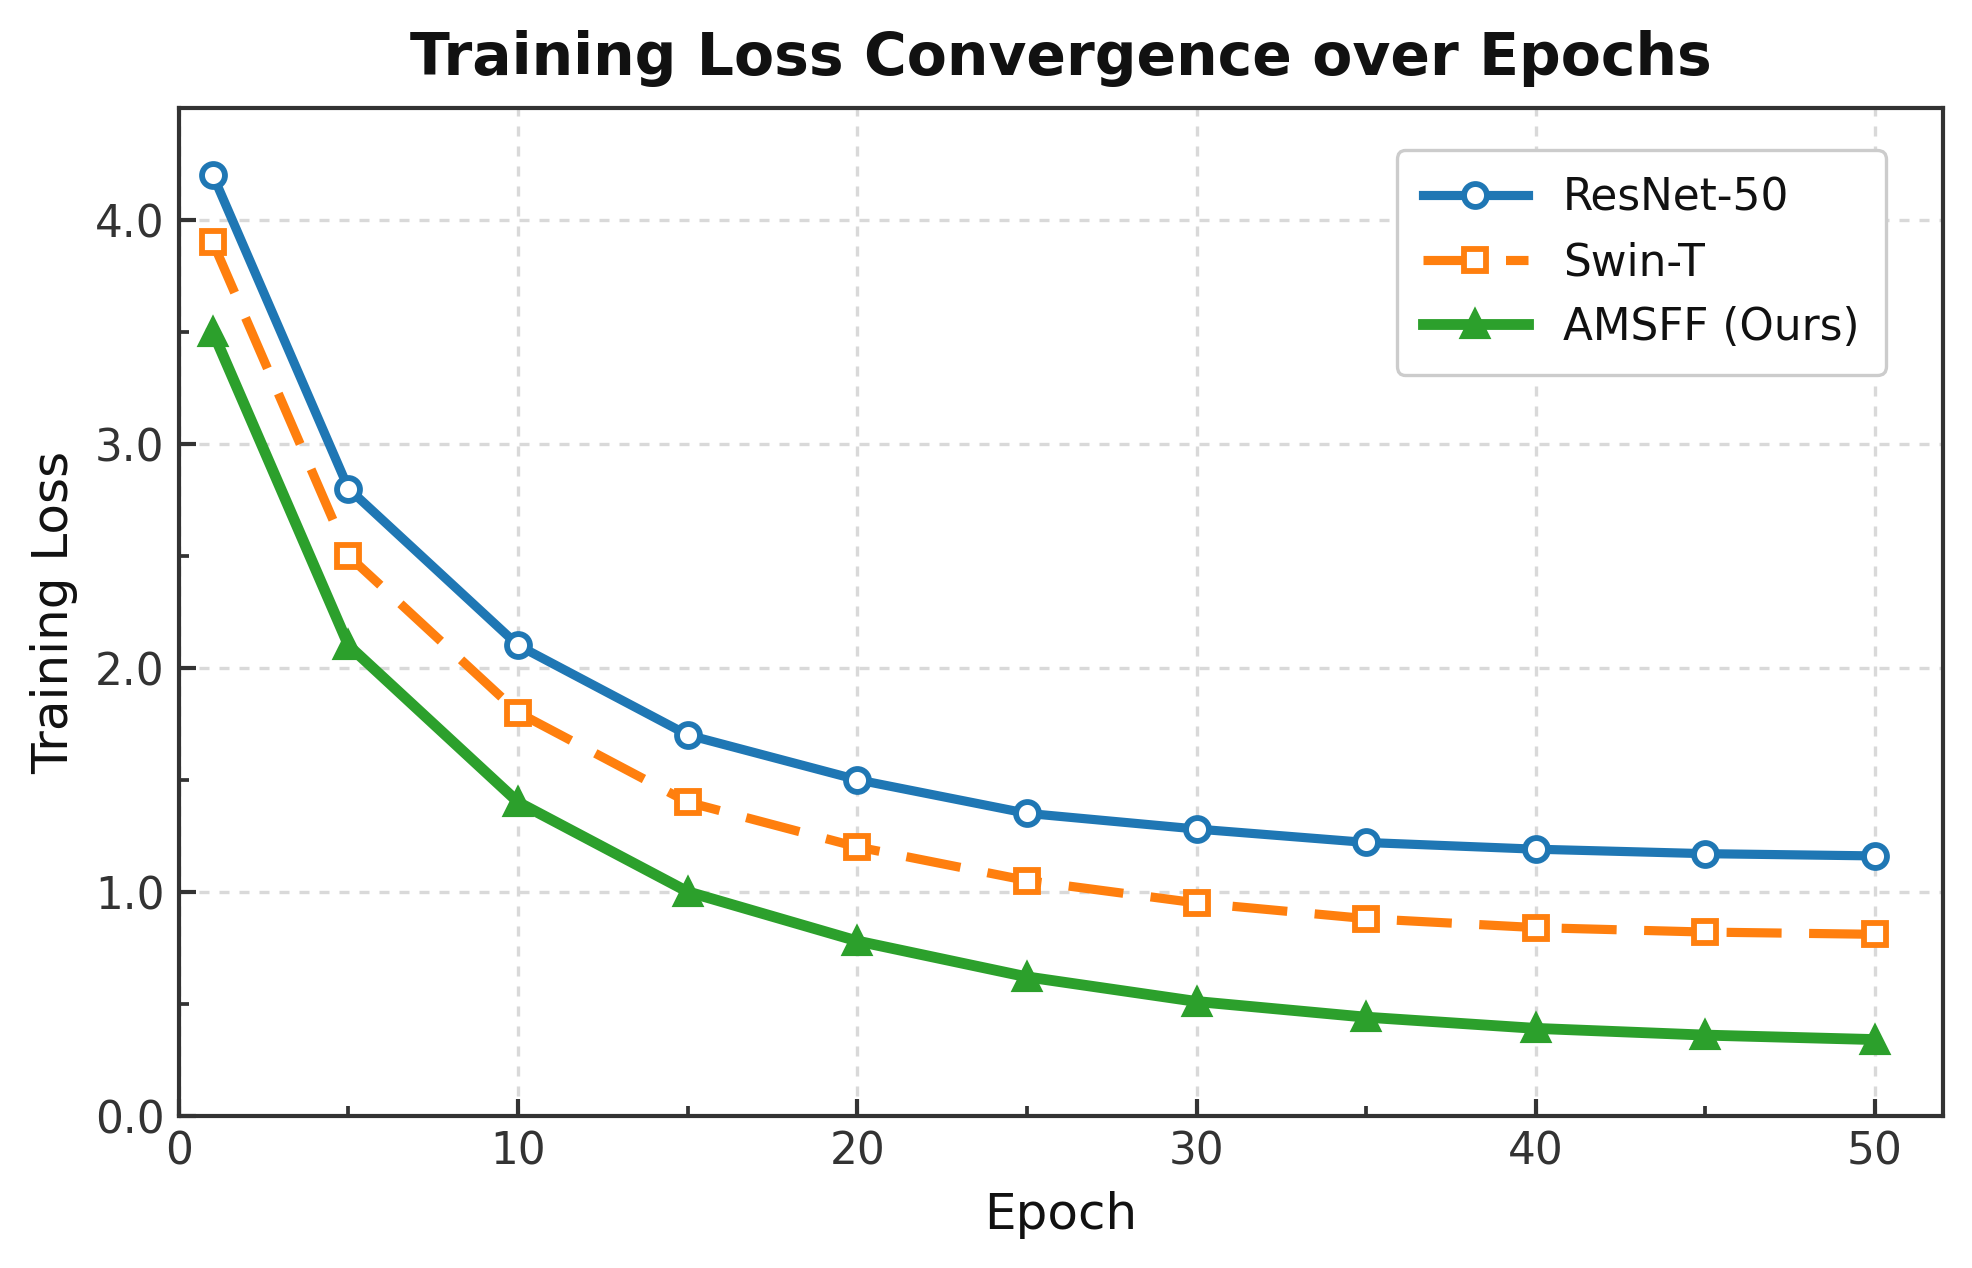
\includegraphics[width=\columnwidth]{convergence.png}
    \caption{Training loss convergence comparison over 50 epochs. AMSFF achieves lower final loss and converges approximately 2.3$\times$ faster than ResNet-50.}
    \label{fig:convergence}
\end{figure}

\subsection{Ablation Study}

\begin{table}[h]
\centering
\caption{Ablation study on AMSFF components.}
\label{tab:ablation}
\begin{tabular}{@{}lcc@{}}
\toprule
\textbf{Configuration} & \textbf{Top-1} & \textbf{mIoU} \\
\midrule
Single-scale (1$\times$ only) & 79.3 & 43.1 \\
+ Multi-scale (concat) & 82.7 & 46.2 \\
+ Cross-Scale Attention & 85.1 & 49.8 \\
+ Scale-Consistency Loss & \textbf{86.4} & \textbf{51.7} \\
\bottomrule
\end{tabular}
\end{table}

Each component contributes meaningfully: multi-scale branches add +3.4\% Top-1, cross-scale attention adds +2.4\%, and scale-consistency loss adds +1.3\%.

\section{Conclusion}

We presented AMSFF, a framework for adaptive multi-scale feature fusion that dynamically attends across resolutions. Our approach achieves state-of-the-art results on both classification and segmentation tasks while converging faster than existing methods. \textit{This demo paper and all its figures were generated entirely by AI using the PaperBanana framework.}

\begin{thebibliography}{9}
\bibitem{lin2017feature} T.-Y. Lin et al., ``Feature Pyramid Networks for Object Detection,'' CVPR, 2017.
\bibitem{yu2015multi} F. Yu and V. Koltun, ``Multi-Scale Context Aggregation by Dilated Convolutions,'' ICLR, 2016.
\bibitem{chen2018encoder} L.-C. Chen et al., ``Encoder-Decoder with Atrous Separable Convolution for Semantic Image Segmentation,'' ECCV, 2018.
\end{thebibliography}

\end{document}
